\documentclass{beamer}
% for handouts: \documentclass[handout]{beamer}

%\setbeamertemplate{background canvas}[vertical shading][bottom=white,top=structure.fg!25]
% or whatever

\usetheme[compress]{Amsterdam}
%\setbeamertemplate{headline}{}
%\setbeamertemplate{footline}{}
%\setbeamersize{text margin left=0.5cm}
  
\usepackage[english]{babel}
\usepackage{listings}
\usepackage{geometry}
\usepackage{hyperref}

\usepackage{color}
%\usepackage[T1]{fontenc}
\usepackage[utf8]{inputenc}
\usepackage{lmodern}

\lstset{
basicstyle=\scriptsize\ttfamily,
columns=flexible,
breaklines=true,
numbers=left,
%stepsize=1,
numberstyle=\tiny,
backgroundcolor=\color[rgb]{0.85,0.90,1}
}




\title[Big Data and Automated Content Analysis]{\textbf{Big Data and Automated Content Analysis} \\ Week 2 -- Thursday \\ Discussing solution Appendix A}
\author[Damian Trilling]{Damian Trilling \\ ~ \\ \footnotesize{d.c.trilling@uva.nl \\@damian0604} \\ \url{www.damiantrilling.net}}
\date{9 April 2020}
\institute[UvA]{Afdeling Communicatiewetenschap \\Universiteit van Amsterdam}

\begin{document}

\begin{frame}{}
\titlepage
\end{frame}

\begin{frame}{Today}
\tableofcontents
\end{frame}



\section{Last week's exercise}
\subsection{Step by step}
\begin{frame}[plain]
\textbf{This week's exercise}\\
\vspace{1cm}
Discussing the code
\end{frame}



\begin{frame}[fragile]{Reading a JSON file into a dict, looping over the dict}
Task 1: Print all titles of all videos
\begin{lstlisting}
import json

with open("/home/damian/pornexercise/xhamster.json") as fi:
    data=json.load(fi)

for k,v in data.items()):
    print (v["title"])
            
\end{lstlisting}
\onslide<2->{
\footnotesize{NB: You have to know (e.g., by reading the documentation of the dataset) that the key is called \texttt{title}}}
\onslide<3->{\\
\footnotesize{NB: \texttt{data} is in fact a dict of dicts, such that each value \texttt{v} is another dict.\\ For each of these dicts, we retrieve the value that corresponds to the key \texttt{title}}}
\end{frame}


\begin{frame}[fragile]{What to do if you do not know the structure of the dataset?}
	Inspecting your data: use the functions \texttt{type()} and \texttt{len()} and/or the dictionary method \texttt{.keys()}
\begin{lstlisting}
len(data)
type(data)
data.keys()
\end{lstlisting}
	\onslide<2->{
		\footnotesize{\texttt{len()} returns the number of items of an object; \texttt{type()} returns the type object; \texttt{.keys()} returns a list of all available keys in the dictionary}}
\end{frame}


\begin{frame}[fragile]{What to do if you do not know the structure of the dataset?}
Inspecting your data: use the module \texttt{pprint} 
\begin{lstlisting}
from pprint import pprint
pprint(data)
\end{lstlisting}

(but better do this on a smaller subset of the data!)
\end{frame}


\begin{frame}[plain]{}
	\makebox[\linewidth]{
		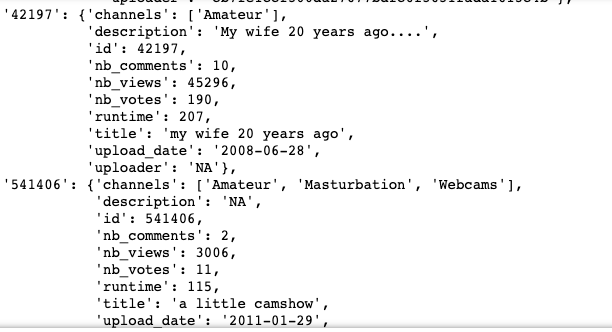
\includegraphics[width=\paperwidth,height=\paperheight,keepaspectratio]{../../pictures/pprint.png}
	}
\end{frame}

\begin{frame}[plain]{}
	\makebox[\linewidth]{
		\includegraphics[width=\paperwidth,height=\paperheight,keepaspectratio]{../../pictures/spyder-dictofdicts.png}
	}
\end{frame}


\begin{frame}[fragile]{For the sake of completeness\ldots}
\texttt{.items()} returns a key-value \emph{pair}, that's why we need to assign \emph{two} variables in the for statement.

These alternatives would also work:
\begin{lstlisting}
for v in data.values()):
	print(v["title"])
\end{lstlisting}

\begin{lstlisting}
for k in data:      #or: for k in data.keys():
	print(data[k]["title"])
\end{lstlisting}

\textbf{Do you see (dis-)advantages?}
\end{frame}



\begin{frame}[fragile]{Working with a subset of the data}
	
What to do if you want to work with a smaller subset of the data?

Taking a random sample of 10 items in a dict:
	\begin{lstlisting}
import random
mydict_short = dict(random.sample(mydict.items(),10))
	\end{lstlisting}
	
Taking the first 10 elements in a list:
	\begin{lstlisting}
mylist_short = mylist[:10]
	\end{lstlisting}

\end{frame}




\begin{frame}[fragile]{Initializing variables, merging two lists, using a counter}
Task 2: Average tags per video and most frequently used tags
\begin{lstlisting}
from collections import Counter
    
alltags=[]
i=0
for k,v in data.items():
    i+=1
    alltags.extend(v["channels"])

print(len(alltags),"tags are describing",i,"different videos")
print("Thus, we have an average of",len(alltags)/i,"tags per video")

c=Counter(alltags)
print (c.most_common(100))
\end{lstlisting}
\scriptsize{(there are other, more efficient ways of doing this)}

\end{frame}





\begin{frame}[fragile]{Nesting blocks, using a defaultdict to count, error handling}
Task 3: What porn category is most frequently commented on?
\begin{lstlisting}
from collections import defaultdict

commentspercat=defaultdict(int)
for k,v in data.items():
        for tag in v["channels"]:
            try:
                commentspercat[tag]+=int(v["nb_comments"])
            except:
                pass
print(commentspercat)
# if you want to print in a fancy way, you can do it like this:
for tag in sorted(commentspercat, key=commentspercat.get, reverse=True):
    print( tag,"\t", commentspercat[tag])
\end{lstlisting}
\scriptsize{A defaultdict is a normal dict, with the difference that the type of each value is pre-defined and it doesn't give an error if you look up a non-existing key}
\onslide<2->{\\~\\
\scriptsize{NB: In line 7, we assume the value to be an int, but the datasets sometimes contains the string ``NA'' instead of a string representing an int. That's why we need the try/except construction}}

\end{frame}



\begin{frame}[fragile]{Adding elements to a list, sum() and len()}
Task 4: Average length of descriptions
\begin{lstlisting}
length=[]
for k,v in data.items():
    length.append(len(v["description"]))
    
print ("Average length",sum(length)/len(length))
\end{lstlisting}

\end{frame}


\begin{frame}[fragile]{Extending (merging) vs appending}
Merging:
\begin{lstlisting}
l1 = [1,2,3]
l2 = [4,5,6]
# either:
l1 = l1 + l2
# or:
l1.extend(l2)
print(l1)
\end{lstlisting}
gives \texttt{[1,2,3,4,5,6]}
~\\

Appending:
\begin{lstlisting}
l1 = [1,2,3]
l2 = [4,5,6]
l1.append(l2)
print(l1)
\end{lstlisting}
gives \texttt{[1,2,3,[4,5,6]]}

\texttt{l2} is seen as \emph{one} element to append to \texttt{l1}
\end{frame}


\begin{frame}[fragile]{Tokenizing with .split()}
Task 5: Most frequently used words
\begin{lstlisting}
allwords=[]
for k,v in data.items():
    allwords+=v["description"].split()
c2=Counter(allwords)
print(c2.most_common(100))
\end{lstlisting}
\scriptsize{
\texttt{.split()} changes a string to a list of words.\\ \texttt{"This is cool''.split()} \\results in\\ \texttt{$[$"This", "is", "cool"$]$}\\
}
\end{frame}


\subsection{Concluding remarks}
\begin{frame}{Concluding remarks}
Make sure you fully understand the code!\\
\vspace{1cm}
Re-read the corresponding chapters\\
\vspace{1cm}
\textbf{PLAY AROUND!!!}\\
\end{frame}


\end{document}

